\documentclass[border=4pt]{standalone}
\usepackage{tikz}
\usepackage{amsmath}
\usetikzlibrary{arrows.meta,positioning,fit,backgrounds}
\begin{document}
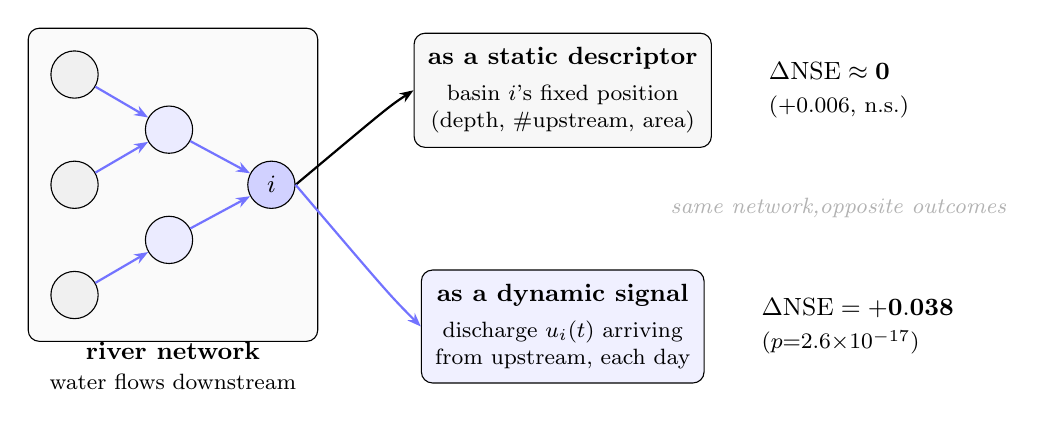
\begin{tikzpicture}[
  font=\small,
  basin/.style={circle,draw,minimum size=6mm,inner sep=0pt,fill=blue!8},
  hb/.style={circle,draw,minimum size=6mm,inner sep=0pt,fill=gray!12},
  flow/.style={-{Stealth[length=5pt]},thick,blue!55},
  box/.style={rounded corners,draw,align=center,inner sep=5pt},
]

% ---------- left: the shared river network ----------
\node[hb] (h1) at (0,1.7) {};
\node[hb] (h2) at (0,0.3) {};
\node[basin] (m1) at (1.2,1.0) {};
\node[hb] (h3) at (0,-1.1) {};
\node[basin] (m2) at (1.2,-0.4) {};
\node[basin,fill=blue!18] (out) at (2.5,0.3) {$i$};
\draw[flow] (h1)--(m1); \draw[flow] (h2)--(m1);
\draw[flow] (m1)--(out); \draw[flow] (m2)--(out);
\draw[flow] (h3)--(m2);
\node[align=center] at (1.25,-2.0) {\textbf{river network}\\\footnotesize water flows downstream};
\begin{scope}[on background layer]
  \node[box,fill=gray!4,fit=(h1)(h3)(out),inner sep=8pt] {};
\end{scope}

% ---------- two forms ----------
\node[box,fill=gray!6] (label) at (6.2,1.5)
  {\textbf{as a static descriptor}\\[2pt]
   \footnotesize basin $i$'s fixed position\\[-1pt]
   \footnotesize (depth, \#upstream, area)};
\node[box,fill=blue!6] (flowbox) at (6.2,-1.5)
  {\textbf{as a dynamic signal}\\[2pt]
   \footnotesize discharge $u_i(t)$ arriving\\[-1pt]
   \footnotesize from upstream, each day};

\draw[-{Stealth[length=5pt]},thick] (out.east) .. controls (4,1.3) .. (label.west);
\draw[-{Stealth[length=5pt]},thick,blue!55] (out.east) .. controls (4,-1.1) .. (flowbox.west);

% ---------- outcomes ----------
\node[align=left,right=6mm of label] (r1)
  {$\Delta\text{NSE} \approx \mathbf{0}$\\[1pt] \footnotesize ($+0.006$, n.s.)};
\node[align=left,right=6mm of flowbox] (r2)
  {$\Delta\text{NSE} = \mathbf{+0.038}$\\[1pt] \footnotesize ($p{=}2.6{\times}10^{-17}$)};
\node[gray!60,font=\footnotesize\itshape] at (9.7,0) {same network,\\opposite outcomes};

\end{tikzpicture}
\end{document}
